\section{Closed-loop Data-enabled Predictive Control}
This section will first present the new \ac{CL-DeePC} framework, which does not suffer from closed-loop identification bias during operation. Subsequently, data equations that underpin this method are derived upon which a noise mitigation strategy using \ac{IVs} is presented.

% ==============================================================================================================================================================
% ==============================================================================================================================================================
\subsection{The basic idea}
To derive a variant of \ac{DeePC} that does not suffer from the aforementioned closed-loop identification issue lets start by considering regular \ac{DeePC}. As mentioned before, closed-loop identification bias can be avoided by using a step-ahead predictor~\cite{Ljung1996}. However, such a short prediction horizon length is typically not conducive to good performance in a receding horizon control setting. Hence, to obtain another output prediction, lets repeat the previous regular \ac{DeePC} problem with the same past data (but a different vector $g$ to span it) to obtain trajectories of input-output data that are shifted forwards one time step. This procedure can be repeated to obtain a desired prediction horizon length $f$. The entire procedure is succinctly described by\todo{check length conditions DeePC}
% 
% To explain the newly-developed \ac{CL-DeePC} framework, consider applying regular \ac{DeePC} $f$ times to the same past data to find consecutive step-ahead predictions of the outputs. This is succinctly described by
% 
\begin{align}\label{eq:CL_DeePC_no_IVs}
\begin{bmatrix}
    U_{i,p,N}\\U_{i_p,1,N}\\Y_{i,p,N}\\ \hline Y_{i_p,1,N}
\end{bmatrix}
\underbrace{
\begin{bmatrix}
    g_1 & g_2 & \cdots & g_f
\end{bmatrix}}_{= G} =
\begin{bmatrix}
    U_{\hat{i},p,f}\\
    U_{\hat{i}_p,1,f}\\
    \widetilde{Y}_{\hat{i},p,f}\\
    \hline
    \widehat{Y}_{\hat{i}_p,1,f}
\end{bmatrix},
% \begin{bmatrix}
%     \datavec{u}{\hat{i},p} & \datavec{u}{\hat{i}+1,p} & \cdots & \datavec{u}{\hat{i}+f-1,p}\\
%     \datavec{u}{\hat{i}_p,1} & \datavec{u}{\hat{i}_p+1,1} & \cdots & \datavec{u}{\hat{i}_p+f-1,1}\\
%     \datavec{y}{\hat{i},p} & \datavec{y}{\hat{i}+1,p} & \cdots & \datavec{y}{\hat{i}+f-1,p}\\
%     \datavec{y}{\hat{i}_p,1} & \datavec{y}{\hat{i}_p+1,1} & \cdots & \datavec{y}{\hat{i}_p+f-1,1}
% \end{bmatrix}
\end{align}
in which $i$, $i_p$, $\hat{i}$, and $\hat{i}_p=\hat{i}+p$ are discrete time indices (the first three indices lie in the past, and the last index $\hat{i}_p$ resembles the first future time index), and $G$ defines a matrix with columns given by the vectors $\{g_k\}^f_{k=1}$. Furthermore, note that $\mathcal{Z}_{i,1,N}$ and $\mathcal{Z}_{\hat{i},1,f}$ are present on respectively the top left and top right hand side.

Treatment of different \ac{CL-DeePC} solution strategies is deferred to Section \ref{sec:SolutionMethods}. Suffice it for now to take note of the structure of \eqref{eq:CL_DeePC_no_IVs} illustrated by Fig.~\ref{fig:CL-DeePC} and to say that if the input is sufficiently persistently exciting such that $\mathcal{Z}_{i,1,N}$ is full row rank~\cite[Chapt.~9.6.1]{Verhaegen2007a} then making $\mathcal{Z}_{i,1,N}$ square and invertible by selecting $N=(p+1)r+pl$ minimizes the number of optimization variables.
% 
% As with regular \ac{DeePC} the idea is to find an optimal combination of allowable future inputs and outputs that minimizes a cost function that is possibly subject to constraints. To see how \eqref{eq:CL_DeePC_no_IVs} can be used in a receding horizon optimal control setting, first consider the top three blocks of the past data matrix. If the input is sufficiently persistently exciting then this matrix, $\mathcal{Z}_{i,1,N}$, is full row rank~\cite[Chapt.~9.6.1]{Verhaegen2007a}. If, furthermore, ${N=(p+1)r+pl}$, then $\mathcal{Z}_{i,1,N}$ becomes square and invertible. Hence, a unique solution for $G$ can then be obtained from the top three block equations of \eqref{eq:CL_DeePC_no_IVs} (in terms of future inputs and outputs), which can then be used to obtain output predictions by using the bottom block equation. The structure of \eqref{eq:CL_DeePC_no_IVs} is visualized by Fig.~\ref{fig:CL-DeePC}. This figure demonstrates that successive future output predictions are dependent on preceding input-output data as well as their concurrent input, opening the door to the sequential construction of an output predictor. This is described in \todo{section}, and can be used in a receding horizon optimal control framework.
% 
\begin{figure}[b!]
\centering
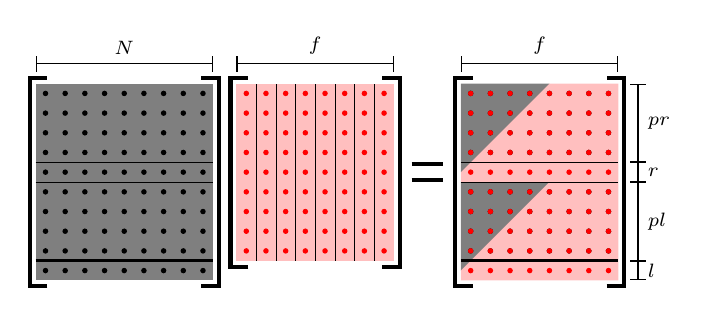
\begin{tikzpicture}
    % defining constants
    \def\stepSize{0.25}
    \def\Nnum{9}
    \def\fnum{8}
    \def\pnum{4}
    
    % Defining lengths
    \newlength{\onelen}
    \setlength{\onelen}{\stepSize cm}
    \newlength{\BrCl}
    \setlength{\BrCl}{0.075cm}
    \newlength{\BrIn}
    \setlength{\BrIn}{0.15cm}
    \newlength{\plen}
    \setlength{\plen}{1cm}%{\pnum\stepSize cm}
    \newlength{\flen}
    \setlength{\flen}{2cm}%{\fnum*\stepSize cm}
    \newlength{\Nlen}
    \setlength{\Nlen}{2.25cm}%{\Nnum\stepSize cm}%should be 2*p+one
    \newlength{\MatClearance}
    \setlength{\MatClearance}{0.3cm}
    
    % grid lines for guidance
    % \draw[gray,step=0.5] (-0,-1) grid (9,3);

    % ======================= drawing data matrix =======================
    \path (0,-\onelen) coordinate (M1A);
    \path ([xshift=\Nlen]M1A) coordinate (M1B);
    \path ([yshift=2*\plen+2*\onelen]M1B) coordinate (M1C);
    \path ([xshift=-\Nlen]M1C) coordinate (M1D);
    \draw[line width=1.5pt] ([xshift=\BrIn,yshift=-\BrCl]M1A) -- ([xshift=-\BrCl,yshift=-\BrCl]M1A) -- ([xshift=-\BrCl,yshift=\BrCl]M1D) -- ([xshift=\BrIn,yshift=\BrCl]M1D); %left bracket
    \draw[line width=1.5pt] ([xshift=-\BrIn,yshift=-\BrCl]M1B) -- ([xshift=\BrCl,yshift=-\BrCl]M1B) -- ([xshift=\BrCl,yshift=\BrCl]M1C) -- ([xshift=-\BrIn,yshift=\BrCl]M1C); %right bracket
    \draw[line width=1pt] ([yshift=\onelen]M1A) -- ([yshift=\onelen]M1B); % dividing matrix into blocks
    \fill[black, opacity=0.5] (M1A) rectangle (M1C);
    \foreach \x in {0,...,8} { % drawing black dots
    \foreach \y in {-1,...,8} {
      \fill ( {(\x+0.5)*\onelen}, {(\y+0.5)*\onelen} ) circle (1pt);
    }}
    \draw[line width=0.1pt] ([yshift=-\plen-\onelen]M1D) -- ([yshift=-\plen-\onelen]M1C);
    \draw[line width=0.1pt] ([yshift=-\plen]M1D) -- ([yshift=-\plen]M1C);
    
    % ======================= drawing G =======================
    % useful coordinates
    \path ([xshift=\MatClearance,yshift=\onelen]M1B) coordinate (M2A);
    \path ([xshift=\flen]M2A) coordinate (M2B);
    \path ([yshift=\Nlen]M2B) coordinate (M2C);
    \path ([xshift=-\flen]M2C) coordinate (M2D);

    % brackets
    \draw[line width=1.5pt] ([xshift=\BrIn,yshift=-\BrCl]M2A) -- ([xshift=-\BrCl,yshift=-\BrCl]M2A) -- ([xshift=-\BrCl,yshift=\BrCl]M2D) -- ([xshift=\BrIn,yshift=\BrCl]M2D); %left bracket
    \draw[line width=1.5pt] ([xshift=-\BrIn,yshift=-\BrCl]M2B) -- ([xshift=\BrCl,yshift=-\BrCl]M2B) -- ([xshift=\BrCl,yshift=\BrCl]M2C) -- ([xshift=-\BrIn,yshift=\BrCl]M2C); %right bracket
    
    % red fill
    \fill[red!50,opacity=0.5] (M2A) rectangle (M2C);

    % drawing red dots
    \foreach \x in {0,...,7} {
    \foreach \y in {0,...,8} {
      \fill[red] ([xshift=(\x+0.5)*\onelen,yshift=(\y+0.5)*\onelen]M2A) circle (1pt);%{(\x+0.5)*\onelen+\Nlen+0.5cm}, {(\y+0.5)*\onelen}
    }}

    % dividers
    \foreach \x in {1,...,7}{\draw[line width=0.1pt] ([xshift=\x*\onelen]M2A) -- ([xshift=\x*\onelen]M2D);}
    
    % ======================= drawing equal sign ======================= 
    \path ([xshift=\MatClearance*3/4,yshift=\Nlen/2-0.1cm]M2B) coordinate (EqA);
    \path ([xshift=0.4cm]EqA) coordinate (EqB);
    \path ([yshift=0.2cm]EqB) coordinate (EqC);
    \path ([xshift=-0.4cm]EqC) coordinate (EqD);
    \draw[line width = 1.5 pt] (EqA) -- (EqB);
    \draw[line width = 1.5 pt] (EqD) -- (EqC);

    % ======================= drawing RHS =======================
    % inside of matrix
    \path ([xshift=\MatClearance*3/4,yshift=-\Nlen/2+0.1cm-\onelen]EqB) coordinate (M3A);
    \path ([xshift=\flen]M3A) coordinate (M3B);
    \path ([yshift=2*\plen+2*\onelen]M3B) coordinate (M3C);
    \path ([xshift=-\flen]M3C) coordinate (M3D);
    % top left black triangle
    \path ([yshift=-\plen-\onelen/2]M3D) coordinate (t1A);
    \path ([xshift=\plen+\onelen/2]M3D) coordinate (t1B);
    % top red trapezoid
    \path ([yshift=-\onelen/2]t1A) coordinate (t2A);
    \path ([xshift=\flen]t2A) coordinate (t2B);
    % bottom black triangle
    \path ([yshift=-\plen-\onelen/2]t2A) coordinate (t3A);
    \path ([xshift=\plen+\onelen/2]t2A) coordinate (t3B);
    % bottom red trapezoid
    \path ([yshift=-\onelen/2]t3A) coordinate (t4A);

    % fill figures
    \fill[black, opacity=0.5]  (t1A) -- (t1B) -- (M3D) -- cycle;% top black
    \fill[red!50, opacity=0.5] (t2A) -- (t2B) -- (M3C) -- (t1B) -- (t1A) -- cycle;% top red
    \fill[black, opacity=0.5]  (t3A) -- (t3B) -- (t2A) -- cycle;% bottom black
    \fill[red!50, opacity=0.5] (t4A) -- (M3B) -- (t2B) -- (t3B) -- (t3A) -- cycle; % bottom red
    
    % draw brackets
    \draw[line width=1.5pt] ([xshift=\BrIn,yshift=-\BrCl]M3A) -- ([xshift=-\BrCl,yshift=-\BrCl]M3A) -- ([xshift=-\BrCl,yshift=\BrCl]M3D) -- ([xshift=\BrIn,yshift=\BrCl]M3D); %left bracket
    \draw[line width=1.5pt] ([xshift=-\BrIn,yshift=-\BrCl]M3B) -- ([xshift=\BrCl,yshift=-\BrCl]M3B) -- ([xshift=\BrCl,yshift=\BrCl]M3C) -- ([xshift=-\BrIn,yshift=\BrCl]M3C); %right bracket
    \draw[line width=1pt] ([yshift=\onelen]M3A) -- ([yshift=\onelen]M3B);
    
    % U_{i,p,N}
    \path ([xshift=0.5*\onelen,yshift=-\plen+0.5*\onelen]M3D) coordinate (tlbA);
    \foreach \x in {0,...,7}{
    \foreach \y in {0,...,3}{
        \ifthenelse{{\y>\x}\OR{\y=\x}}{%
        \fill[black] ([xshift={\x*\onelen},yshift={\y*\onelen}]tlbA) circle (1pt);%<do this if true>
        }{%
        \fill[red] ([xshift={\x*\onelen},yshift={(\y*\onelen}]tlbA) circle (1pt);%<do this if false>
        }%
    }}
    
    % U_{i_p,1,N}
    \path ([yshift=-\onelen]tlbA) coordinate (tlbB);
    \foreach \x in {0,...,7}{\fill[red] ([xshift=\x*\onelen]tlbB) circle (1pt);}
    
    % Y_{i,p,N}
    \path ([yshift=-\plen]tlbB) coordinate (tlbC);
    \foreach \x in {0,...,7}{
    \foreach \y in {0,...,3}{
        \ifthenelse{{\y>\x}\OR{\y=\x}}{%
        \fill[black] ([xshift={\x*\onelen},yshift={\y*\onelen}]tlbC) circle (1pt);%<do this if true>
        }{%
        \fill[red] ([xshift={\x*\onelen},yshift={(\y*\onelen}]tlbC) circle (1pt);%<do this if false>
        }%
    }}

    % Y_{i_p,1,N}
    \path ([yshift=-\onelen]tlbC) coordinate (tlbD);
    \foreach \x in {0,...,7}{\fill[red] ([xshift=\x*\onelen]tlbD) circle (1pt);}

    % draw dividers
    \draw[line width=0.1pt] ([yshift=-\plen-\onelen]M3D) -- ([yshift=-\plen-\onelen]M3C);
    \draw[line width=0.1pt] ([yshift=-\plen]M3D) -- ([yshift=-\plen]M3C);

    % ======================= length indicators ======================= 
    \draw[|-|] ([yshift=\onelen]M1D) -- node[above] {\scriptsize$N$} ([yshift=\onelen]M1C);
    \draw[|-|] ([yshift=\onelen]M2D) -- node[above] {\scriptsize$f$} ([yshift=\onelen]M2C);
    \draw[|-|] ([yshift=\onelen]M3D) -- node[above] {\scriptsize$f$} ([yshift=\onelen]M3C);
    \draw[|-|] ([xshift=\onelen]M3C) -- node[right] {\scriptsize$pr$} ([xshift=\onelen,yshift=\onelen]t2B);
    \draw[|-|] ([xshift=\onelen,yshift=\onelen]t2B) -- node[right] {\scriptsize$r$} ([xshift=\onelen]t2B);
    \draw[|-|] ([xshift=\onelen]t2B) -- node[right] {\scriptsize$pl$} ([xshift=\onelen,yshift=\onelen]M3B);
    \draw[|-|] ([xshift=\onelen,yshift=\onelen]M3B) -- node[right] {\scriptsize$l$} ([xshift=\onelen]M3B);
\end{tikzpicture}
\caption{Visualization of known (black) and unknown (red) variables in \ac{CL-DeePC}. Each dot represents an input $u_k\in\mathbb{R}^r$, output $y_k\in\mathbb{R}^l$, or element of the matrix $G$.
Note that block-anti-diagonals of inputs or outputs are composed of a single time sample. Without \ac{IVs}, as in \eqref{eq:CL_DeePC_no_IVs}, $m=N$, whilst with \ac{IVs}, as in \eqref{eq:CL_DeePC_IV}, $m=(p+1)r+pl$.}
\label{fig:CL-DeePC}
\end{figure}

% ==============================================================================================================================================================
% ==============================================================================================================================================================
\subsection{The data equations}
To motivate a noise mitigation strategy based that is based on \ac{IVs} that is explained hereafter, the data equations that justify this approach are first derived here using a state-space approach.

To this end, it is straightforward to show by iterative application of respectively \eqref{eqn:SS_innovation} and \eqref{eqn:SS_predictor} that%
\begin{align}
    Y_{i_p,s,N} &= \Gamma_s X_{i_p,1,N} + \mathcal{T}_s^\mathrm{u} U_{i_p,s,N} + \mathcal{H}_s E_{i_p,s,N}\label{eq:Yf1},\\
    \begin{split}%
    Y_{i_p,s,N} &= \widetilde{\Gamma}_s X_{i_p,1,N} + \widetilde{\mathcal{T}}_s^\mathrm{u} U_{i_p,s,N} + E_{i_p,s,N}\\
    &\phantom{=}+(I_{sl}-\widetilde{\mathcal{H}}_s)Y_{i_p,s,N},
    \end{split}\label{eq:Yf2}
\end{align}
in which $s\in\mathbb{Z}^+$ represents a window length. It is possible to rewrite the initial states in terms of preceding states and input-output data using \eqref{eqn:SS_predictor} as%
\begin{align}\label{eq:Xip}
    X_{i_p,1,N} = \tilde{A}^p X_{i,1,N} + \tKp{u} U_{i,p,N} + \tKp{y} Y_{i,p,N}.
    % \begin{bmatrix}
    %     Y_{i,p,N}\\
    %     U_{i,p,N}
    % \end{bmatrix}.
\end{align}
% in which $\tKp{}=\big[\tKp{y}\;\;\tKp{u}\big]$.
By the existence of \eqref{eqn:SS_innovation} with a stabilizing Kalman gain $K$, $\tilde{A}$ must have all eigenvalues inside the unit circle. Assuming a sufficiently large $p$ such that $\tilde{A}^p\approx 0$ (a common assumption in subspace methods~\cite{Chiuso2007}) substitute \eqref{eq:Xip} into \eqref{eq:Yf1} and \eqref{eq:Yf2} to obtain two so called data equations:
\begin{align}
    Y_{i_p,s,N} &= L_s \mathcal{Z}_{i,s,N} + \mathcal{H}_s E_{i_p,s,N}\label{eq:DataEq1}\\
    Y_{i_p,s,N} &= \widetilde{L}_s \mathcal{Z}_{i,s,N} + (I_{sl}-\widetilde{\mathcal{H}}_s) Y_{i_p,s,N} + E_{i_p,s,N},\label{eq:DataEq2}
\end{align}
in which $L_s$, $\widetilde{L}_s$, $\mathcal{Z}_{i,s,N}$ are defined in Section \ref{sec:notation}. Similarly to \eqref{eq:DataEq1} and \eqref{eq:DataEq2}, the future outputs are defined by
\todo{use noiseless?}%always refer to noiseless version or beter to refer to ideal predictor here?
\begin{align}
    Y_{\hat{i}_p,s,f} &= L_s \mathcal{Z}_{\hat{i},s,f} + \mathcal{H}_s E_{\hat{i}_p,s,f},\label{eq:DataEq1.2}\\
    Y_{\hat{i}_p,s,f} &= \widetilde{L}_s \mathcal{Z}_{\hat{i},s,f} + (I_{sl}-\widetilde{\mathcal{H}}_s) Y_{\hat{i}_p,s,f} + E_{\hat{i}_p,s,f}\label{eq:DataEq2.2}.
\end{align}
Although a more generic representation was kept above for later analysis, for \ac{CL-DeePC}, $s=1$. This reduces the complexity of the above equations since ${\widetilde{L}_1=L_1=\big[ C\tKp{u} \; D \; C\tKp{y} \big]}$ and $\widetilde{\mathcal{H}}_1=\mathcal{H}_1=I_l$.
%
% ==============================================================================================================================================================
% ==============================================================================================================================================================
\subsection{Noise mitigation using \acl{IVs}}
In obtaining an output predictor, no systematic noise mitigation strategy is yet applied by \eqref{eq:CL_DeePC_no_IVs} as the columns of $G$ simply take linear combinations of the noise in the output demonstrated by \eqref{eq:DataEq1}. An altered formulation of \eqref{eq:CL_DeePC_no_IVs} is therefore considered that allows the use of \ac{IVs} ($\mathcal{I}_\mathrm{IV}$) as in~\cite{vanWingerden2022}
\begin{align}\label{eq:CL_DeePC_IV}
    \begin{bmatrix}
   \mathcal{Z}_{i,1,N}\\
   \hline
   Y_{i_p,1,N}
    \end{bmatrix}
{\mathcal{I}_\mathrm{IV}}^\top G =
\begin{bmatrix}
    \mathcal{Z}_{\hat{i},1,f}\\
    \hline
    \widehat{Y}_{\hat{i}_p,1,f}
\end{bmatrix},
\end{align}
in which $G$ may be different from its previous definition depending on the definition of $\mathcal{I}_\mathrm{IV}$, which follows shortly. Note that \eqref{eq:CL_DeePC_no_IVs} is recovered with $\mathcal{I}_\mathrm{IV}=I_N$.

From \eqref{eq:DataEq1} and \eqref{eq:CL_DeePC_IV} the output predictor becomes
\begin{align}\label{eq:OutputPred}
    \widehat{Y}_{\hat{i}_p,1,f} = L_1 \mathcal{Z}_{\hat{i},1,f} + \mathcal{H}_1 E_{i_p,1,N}{\mathcal{I}_\mathrm{IV}}^\top G.
\end{align}
To obtain an output estimate that best resembles a noiseless version of the actual future outputs given by \eqref{eq:DataEq1.2} it is desirable to reduce the noise contribution on the right hand side above. In addition, from an optimization point of view, it would be favorable to choose an \acs{IV} that uniquely determines $G$ from \eqref{eq:CL_DeePC_IV} given $\mathcal{Z}_{\hat{i},1,f}$ and a sufficiently persistently exciting input that ensures that $\mathcal{Z}_{i,1,N}$ is full row rank.

This motivates choosing $\mathcal{I}_\mathrm{IV}=\mathcal{Z}_{i,1,N}$ as an \acs{IV} since\footnote{Since ${\mathcal{I}_\mathrm{IV}}^\top G$ is fixed by \eqref{eq:CL_DeePC_IV} scalar multiples of the chosen \ac{IV} would be equally valid, simply resulting in a different $G$.}%
\begin{align}
    &\lim_{N\rightarrow\infty} \frac{1}{N}E_{i_p,1,N}{\mathcal{Z}_{i,1,N}}^\top = \mathcal{O},\label{eq:uncorrelated}\\
    \text{rank}\biggl(&\lim_{N\rightarrow\infty} \frac{1}{N}\mathcal{Z}_{i,1,N}{\mathcal{Z}_{i,1,N}}^\top\biggl) =  \text{rank}(\mathcal{Z}_{i,1,N}).\label{eq:rankconservation}
\end{align}
As demonstrated by \eqref{eq:uncorrelated}, the instrumental variable and the noise are uncorrelated\footnote{Note that the choice $s=1$ is essential here to avoid correlation between inputs and noise during operation with data obtained in closed-loop.}. Hence, \eqref{eq:OutputPred} asymptotically converges to an ideal, noiseless output predictor with increasing $N$. In addition, provided that the input is sufficiently persistently exciting, $\mathcal{Z}_{i,1,N}$ is full row rank such that \eqref{eq:rankconservation} permits only a single, unique solution for $G$ in \eqref{eq:CL_DeePC_IV}.